\chapter{Biblioteca Mathematical Components}
\label{cap:mathcomp}

Nos capítulos seguintes será usada uma série de itens disponíveis na biblioteca Mathematical Components e outros implementados com uso da biblioteca. Todavia é necessário, por parte do leitor, um conhecimento básico sobre essa biblioteca, e para isso, neste capítulo serão explicados elementos que foram considerados mais essenciais de acordo com o tema definido. Todo o conteúdo a seguir se baseia em \cite{assia_mahboubi_2022_7118596}.

Ademais, é importante ressaltar que, na apresentação dos conteúdos deste capítulo, se assume que o leitor possui um conhecimento básico sobre \textit{Coq}, e em caso contrário recomenda-se que o leitor acesse o material disponível em: \url{https://softwarefoundations.cis.upenn.edu/lf-current/index.html}

\section{Módulos}
A biblioteca Mathematical Components é divida em módulos, nos quais alguns são simplesmente a união de outros menores relacionados entre si. No site oficial da biblioteca\footnote{\url{https://math-comp.github.io/}} está disponível, além do livro utilizado como referência neste trabalho \cite{assia_mahboubi_2022_7118596}, um grafo
de tais módulos. A Figura \ref{fig:graph-mathcomp} apresenta uma parte desse grafo:

\begin{figure}[h]
        \centering
        \caption{Grafo do módulo ssreflect}
        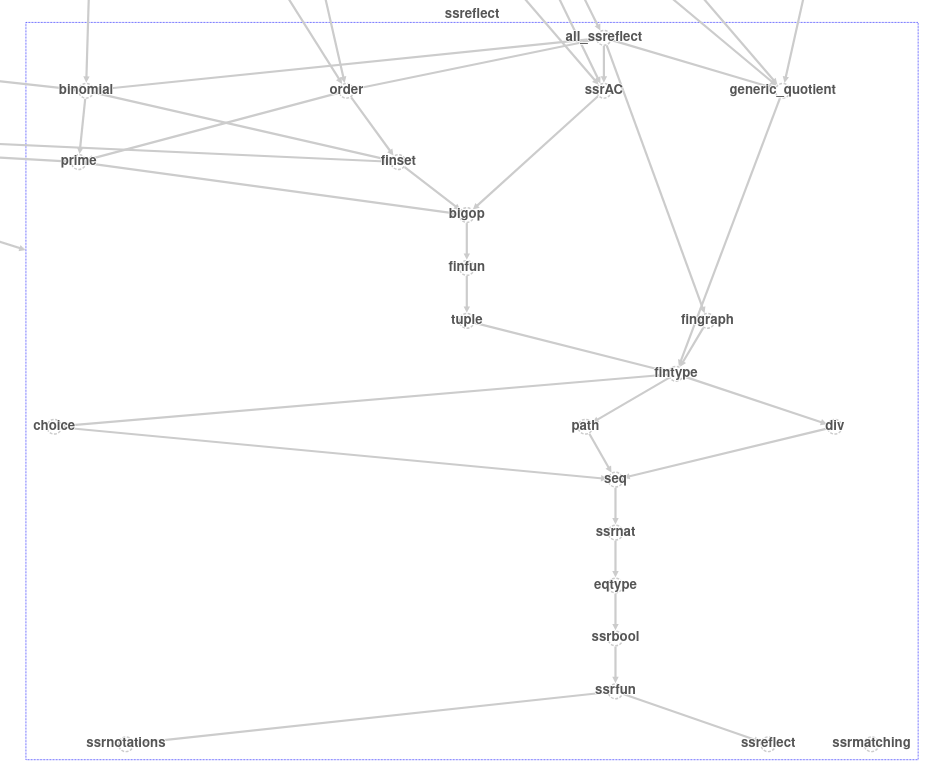
\includegraphics[width=0.6\textwidth]{Figuras/ssreflect.png}\\
        \footnotesize{Disponível em: <\url{https://math-comp.github.io/htmldoc_2_2_0/libgraph.html}>.
        Acesso em: 18 de maio de 2024.}
        \label{fig:graph-mathcomp}
\end{figure}

Os módulos principais para o desenvolvimento da prova sobre o algoritmo Tonelli-Shanks (com base no conteúdo de Teoria dos Números que sustenta a lógica do mesmo) são: \textit{all\_ssreflect} (que contém diversos outros módulos), \textit{ring\_quotient}, \textit{zmodp} e \textit{intdiv}.

\section{Igualdades}
Na maior parte dos teoremas das bibliotecas nativas de \textit{Coq}, usa-se a igualdade de Leibniz. Por sua vez, essa definição de igualdade é dada pela seguinte proposição indutiva (de acordo com a documentação\footnote{\url{https://coq.inria.fr/doc/V8.18.0/refman/proofs/writing-proofs/equality.html}} \cite{coqteam2022manual}):

\begin{lstlisting}[language = coq]
    Inductive eq {A : Type} (x : A) : A -> Prop := eq_refl : eq x x.
\end{lstlisting}

De maneira distinta, a biblioteca Mathematical Components, em suas definições e teoremas, utiliza com frequência predicados booleanos \cite{assia_mahboubi_2022_7118596}, que são basicamente funções cujo tipo de retorno é \lstinline[language = coq]!bool!, para então representar proposições da forma \lstinline[language = coq]$x = true$, onde \lstinline[language = coq]$x$ é uma expressão cujo retorno é do tipo \lstinline[language = coq]!bool!. Tais proposições são construídas pela função \lstinline[language = coq]$is_true$.No entanto, através do comando \lstinline[language = coq]$Coercion$ (que será explicado mais detalhadamente adiante neste documento) e por questões de legibilidade, tal função é omitida e o sistema de tipos de \textit{Coq} é capaz de inferir quando uma expressão deve ter tipo \lstinline[language = coq]$bool$ ou tipo \lstinline[language = coq]$Prop$ (e então há uma aplicação de \lstinline[language = coq]$is_true$ omitida). 

Semelhantes aos teoremas existentes para proposição comuns, estão disponíveis diversos teoremas para proposições geradas com o uso de \lstinline[language = coq]$is_true$, como por exemplo o lema \lstinline[language = coq]$contraLR$. Esse é uma versão da contraposição utilizando predicados booleanos (junto à função \lstinline[language = coq]$is_true$) e sua definição é dada por:
\begin{lstlisting}[language = coq]
        Lemma contraLR (c b : bool) : (~~ c -> ~~ b) -> b -> c.
\end{lstlisting}
onde \lstinline[language = coq]$~~$ é a operação de negação definida na biblioteca Mathematical Components.

Outra informação relevante ao se tratar do conteúdo da biblioteca é o tipo \lstinline[language = coq]$eqType$: para que seja construído qualquer habitante desse tipo é necessário um elemento \lstinline[language = coq]$T$ de tipo 
\lstinline[language = coq]$Type$, uma função \lstinline[language = coq]$eq_op$ de tipo \lstinline[language = coq]$T -> T -> bool$
e um elemento \lstinline[language = coq]$eqP$ cujo tipo é um teorema relacionando a igualdade de Leibniz com \lstinline[language = coq]$T$ e \lstinline[language = coq]$eq_op$. Este último possui, na biblioteca, uma notação de nome \lstinline[language = coq]$eq_axiom$, e sua descrição é:
\begin{lstlisting}[language = coq]
    Definition eq_axiom: forall (T : Type) (e : rel T), forall x x0 : T, 
            reflect (x = x0) (e x x0)
\end{lstlisting}
onde \lstinline[language = coq]$rel T$ é equivalente ao tipo \lstinline[language = coq]$T -> T -> bool$.

Portanto, para que um tipo \lstinline[language = coq]$A$
pertença ao primeiro campo mencionado, é necessário que se tenha uma prova da proposição \lstinline[language = coq]$eq_axiom A$, isto é, 
a definição \lstinline[language = coq]$eq_axiom$ com 
\lstinline[language = coq]$T$ igual a \lstinline[language = coq]$A$.
Tal teorema indica que a igualdade sobre \lstinline[language = coq]$A$
é decidível, o que fica claro pelo seguinte lema:

\begin{lstlisting}[language = coq]
    Lemma decP: forall (P : Prop) (b : bool), reflect P b -> decidable P
\end{lstlisting}

A utilização de um tipo como \lstinline[language = coq]$eqType$ facilita que se provem teoremas genéricos, no sentido de que servem para diferentes tipos (pertencentes a \lstinline[language = coq]$Type$) desde que estes possuam uma relação de equivalência decidível. Existem outros tipos semelhantes a \lstinline[language = coq]$eqType$, no sentido de que servem como interfaces. Em grande parte, esses são implementados por meio do açúcar sintático \lstinline[language = coq]$Record$, qual será explicado na sessão seguinte.

\section{Structures e Records} 
\label{section:structs-e-records}

\lstinline[language = coq]$Structure$ e \lstinline[language = coq]$Record$ são comandos sinônimos para geração de tipos indutivos que possuem somente um construtor e cujo os campos são dependentemente tipados, isto é, o tipo de cada campo pode depender dos valores de campos anteriores, assim como nas definições indutivas \cite{assia_mahboubi_2022_7118596}. A vantagem do uso desses comandos é que por meio desses são geradas automaticamente funções para extrair valores dos argumentos do construtor do tipo declarado.

Estes comandos são frequentemente utilizados na biblioteca Mathematical Components para definir interfaces (como o \lstinline[language = coq]$eqType$) e subtipos (ex.: tipo em que os habitantes são todos os números naturais menores que $8$). Para melhor entendimento do leitor, tem-se a seguir um exemplo semelhante ao tipo \lstinline[language = coq]$eqType$ definido na biblioteca, apresentado em \cite{assia_mahboubi_2022_7118596}:
\begin{lstlisting}[language = coq]
    Record eqType : Type := Pack
    {
        sort : Type;
        eq_op : sort -> sort -> bool;
        axiom : eq_axiom eq_op
    }.
\end{lstlisting}
Como explicado acima, essa declaração é equivalente a se fazer as seguintes declarações:
\begin{lstlisting}[language = coq]
        Inductive eqType : Type :=
            | Pack (sort : Type) (eq_op : sort -> sort -> bool) (axiom : eq_axiom eq_op).
            
        Definition sort (e : eqType) : Type :=
            match e with
            | Pack t _ _ => t
            end.
        Definition eq_op (e : eqType) : (sort e -> sort e -> bool) :=
            match e with
            | Pack _ f _ => f
            end.
        Definition axiom (e : eqType) : (eq_axiom (eq_op e)) :=
            | Pack _ _ a => a
            end.
\end{lstlisting}
Observe que o uso de tipos dependentes ocorre nos campos \lstinline[language = coq]{eq_op} e \lstinline[language = coq]{axiom}. No primeiro, o tipo do campo depende do valor do campo \lstinline[language = coq]{sort} e no segundo o tipo do campo depende do valor do campo \lstinline[language = coq]{eq_op} e portanto também do campo \lstinline[language = coq]{sort}.

\subsection{Comando Canonical} Assim como apresentado em \cite{assia_mahboubi_2022_7118596}, para instanciar um habitante de \lstinline[language = coq]$eqType$ com campo \lstinline[language = coq]$sort$ igual a \lstinline[language = coq]$nat$, deve-se provar o seguinte teorema:
\begin{lstlisting}[language = coq]
    Theorem axiom_nat: eq_axiom eqn.
\end{lstlisting}
onde \lstinline[language = coq]$eqn$ é uma operação de comparação booleana entre números naturais.
Tendo esta prova, podemos instanciar tal habitante
da seguinte forma:
\begin{lstlisting}[language = coq]
    Definition natEqtype := Pack nat eqn axiom_nat.
\end{lstlisting}
Note que, agora, pode-se comparar dois números naturais da seguinte maneira:
\begin{lstlisting}[language = coq]
    Compute (@eq_op natEqType 2 2).
\end{lstlisting}
o que nesse caso equivale a:
\begin{lstlisting}[language = coq]
    Compute (eqn 2 2).
\end{lstlisting}

Entretanto, o objetivo de criar o tipo \lstinline[language = coq]$eqType$ não é estabelecer essa possibilidade de computação para relações de comparação, mas sim construir definições, funções e provas genéricas para todos os tipos que pertencem ao campo \lstinline[language = coq]$sort$ de algum habitante de \lstinline[language = coq]$eqType$ e estabelecer \textit{overloading} de notações. Para exemplo de como alcançar este último objetivo, se define uma notação da seguinte forma:

\begin{lstlisting}[language = coq]
        Notation "x == y" := (@eq_op _ x y).
\end{lstlisting}
porém havendo apenas esta definição, caso executado o comando \lstinline[language = coq]$Check (3 == 2)$ tem-se um falha. Ao se executar:
\begin{lstlisting}[language = coq]
    Fail Check (3 == 2).
\end{lstlisting}
a seguinte mensagem é apresentada:
\begin{lstlisting}[language = coq-error]
    The command has indeed failed with message:
    The term "3" has type "nat" while it is 
    expected to have type "sort ?e"
\end{lstlisting}
Isto ocorre pois o \textit{Coq} não é capaz de inferir o argumento implícito\footnote{Note que o comando \lstinline[language = coq]$Fail Check (3 == 2)$ é equivalente a \lstinline[language = coq]$Fail Check (@eq_op _ 3 2)$.}  (\lstinline[language = coq]$_$).

Note que é mencionada uma variável \lstinline[language = coq]$?e$. Essa representa um elemento a ser inferido de modo que o tipo \lstinline[language = coq]$sort ?e$ seja igual ao tipo \lstinline[language = coq]$nat$. Como exposto em \cite{10.1007/978-3-642-39634-2_5} o algoritmo de inferência do \textit{Coq} não é capaz de descobrir o valor de tal variável por meio das regras de inferência que possui. Para resolver este problema 
o \textit{Coq} permite que se adicione regras de inferência de tipo por meio do comando \lstinline[language = coq]$Canonical$ (que recebe um construtor de algum \lstinline[language = coq]$Record$ ou \lstinline[language = coq]$Structure$ aplicado aos seus argumentos). Assim, resolver esse problema é possível por meio do seguinte código:
\begin{lstlisting}[language = coq]
    Canonical natEqType.
\end{lstlisting}
Com isto, de maneira semelhante ao exemplo exposto em \cite{10.1007/978-3-642-39634-2_5}, é adicionada a seguinte regra de inferência ao algoritmo presente em \textit{Coq}:

\begin{equation*}
        \inferrule 
        {
        \text{\lstinline[language = coq]!nat!} \sim 
        \text{\lstinline[language = coq]!sort natEqType!} 
        \\
        \; \text{\lstinline[language = coq]!?!} \text{\lstinline[language = coq]!e!} \; \sim
        \text{\lstinline[language = coq]!natEqType!} 
        }
        {\text{\lstinline[language = coq]!nat!} \sim \text{\lstinline[language = coq]!sort ?e!}}   
\end{equation*}
em que a notação $\sim$ representa uma chamada do algoritmo de unificação \cite{10.1007/978-3-642-39634-2_5} (que é o nome dado ao algoritmo de comparação de tipos chamado nas rotinas de inferência de tipos). Neste momento o leitor pode se perguntar como tal regra de inferência leva o algoritmo a chegar em um resultado final, e a resposta de acordo \cite{10.1007/978-3-642-39634-2_5} está em na existência de outras regras de inferência, como \textit{eq} e \textit{assign}: